%%%%%%%%%%%%%%%%% DO NOT CHANGE HERE %%%%%%%%%%%%%%%%%%%% 
%%%%%%%%%%%%%%%%%%%%%%%%%%%%%%%%%%%%%%%%%%%%%%%%%%%%%%%%%%{
    \documentclass[twoside,11pt]{article}
    %%%%% PACKAGES %%%%%%
    \usepackage{ctex}
    \usepackage{pgm2016}
    \usepackage{amsmath}
    \usepackage{algorithm}
    \usepackage[noend]{algpseudocode}
    \usepackage{subcaption}
    \usepackage[english]{babel}	
    \usepackage{paralist}	
    \usepackage[lowtilde]{url}
    \usepackage{fixltx2e}
    \usepackage{listings}
    \usepackage{color}
    \usepackage{enumerate}
    \usepackage{booktabs}
    \usepackage{multicol}
    \usepackage{multirow}
    \usepackage{auto-pst-pdf}
    \usepackage{pst-all}
    \usepackage{pstricks-add}
	\usepackage{comment}
	\usepackage{fancybox}
    \usepackage[hidelinks]{hyperref}
    \usepackage{bbding}
    \usepackage{hyperref}
    \usepackage{texnames}

    %%%%% MACROS %%%%%%
    \algrenewcommand\Return{\State \algorithmicreturn{} }
    \algnewcommand{\LineComment}[1]{\State \(\triangleright\) #1}
    \renewcommand{\thesubfigure}{\roman{subfigure}}
    \definecolor{codegreen}{rgb}{0,0.6,0}
    \definecolor{codegray}{rgb}{0.5,0.5,0.5}
    \definecolor{codepurple}{rgb}{0.58,0,0.82}
    \definecolor{backcolour}{rgb}{0.95,0.95,0.92}
    \lstdefinestyle{mystyle}{
       backgroundcolor=\color{backcolour},  
       commentstyle=\color{codegreen},
       keywordstyle=\color{magenta},
       numberstyle=\tiny\color{codegray},
       stringstyle=\color{codepurple},
       basicstyle=\footnotesize,
       breakatwhitespace=false,        
       breaklines=true,                
       captionpos=b,                    
       keepspaces=true,                
       numbers=left,                    
       numbersep=5pt,                  
       showspaces=false,                
       showstringspaces=false,
       showtabs=false,                  
       tabsize=2
    }
    \lstset{style=mystyle}
%%%%%%%%%%%%%%%%%%%%%%%%%%%%%%%%%%%%%%%%%%%%%%%%%%%%%%%%%% 
%%%%%%%%%%%%%%%%%%%%%%%%%%%%%%%%%%%%%%%%%%%%%%%%%%%%%%%%%% }

%%%%%%%%%%%%%%%%%%%%%%%% CHANGE HERE %%%%%%%%%%%%%%%%%%%% 
%%%%%%%%%%%%%%%%%%%%%%%%%%%%%%%%%%%%%%%%%%%%%%%%%%%%%%%%%% {
\newcommand\schoolName{Zhejiang Sci-Tech University}
\newcommand\course{Course Code: 62941-1}
\newcommand\courseName{Human Computer Interaction*}
\newcommand\info{Experiment 1}
%个人信息
\newcommand\studentName{Wang Xugang}
\newcommand\studentEmail{Email: castamerego@gmail.com}
\newcommand\studentNumber{2020329621074}
\newcommand\studentClass{Computer Sci/Tec(English)20(1)}
%%%%%%%%%%%%%%%%%%%%%%%%%%%%%%%%%%%%%%%%%%%%%%%%%%%%%%%%%% }
%%%%%%%%%%%%%%%%%%%%%%%%%%%%%%%%%%%%%%%%%%%%%%%%%%%%%%%%%%

%%%%%%%%%%%%%%%%% DO NOT CHANGE HERE %%%%%%%%%%%%%%%%%%%% 
%%%%%%%%%%%%%%%%%%%%%%%%%%%%%%%%%%%%%%%%%%%%%%%%%%%%%%%%%%
%{
    \renewcommand{\thefootnote}{\fnsymbol{footnote}}
    \newenvironment{boxedlaw}[1]
    {\begin{Sbox}\begin{minipage}{#1}\setcounter{mpfootnote}{\value{footnote}}}
            {\end{minipage}\end{Sbox}\begin{center}\shadowbox{\TheSbox}
            \setcounter{footnote}{\value{mpfootnote}}\end{center}}
    
    \renewcommand*\thempfootnote{\fnsymbol{mpfootnote}}
    
    \ShortHeadings{\schoolName -  ~~ \courseName ~~ \info}{\studentName - \studentNumber}
        \firstpageno{1}
        
\begin{document}

%%%%%%%%%%%%%%%%%%%%%%%% Title %%%%%%%%%%%%%%%%%%%%

\begin{figure}[H]
    \centering
    
\includegraphics[width=1\columnwidth]{figures/zstu-logo.png}
\end{figure}


\title{\Huge \LaTeX  -- Template}

\vspace{1cm}

\author{\name \studentName \email \studentEmail \\
    \studentNumber \class  \studentClass
    \addr
}

\maketitle

\newpage


%%%%%%%%%%%%%%%%%%%%%%%% Author %%%%%%%%%%%%%%%%%%%%

\phantomsection\addcontentsline{toc}{section}{Author}\tolerance=500

\begin{center}
    王旭刚\textsuperscript{1*}

    \bigskip
    \textbf{1*} Author

    \bigskip
    %
\end{center}



%%%%%%%%%%%%%%%%%%%%%%%% Abstruct %%%%%%%%%%%%%%%%%%%%


\phantomsection\addcontentsline{toc}{section}{Abstruct}\tolerance=500

\begin{center}
    \Large\textbf{Abstruct}
\end{center}

Lorem ipsum dolor sit amet, consectetur adipisicing elit, sed do eiusmod tempor incididunt ut labore et dolore magna aliqua. Ut enim ad minim veniam, quis nostrud exercitation ullamco laboris nisi ut aliquip ex ea commodo consequat. Duis aute irure dolor in reprehenderit in voluptate velit esse cillum dolore eu fugiat nulla pariatur. Excepteur sint occaecat cupidatat non proident, sunt in culpa qui officia deserunt mollit anim id est laborum.

\pagenumbering{Roman}
\newpage

%%%%%%%%%%%%%%%%%%%%%%%% 课题执行(文档修订)记录表 %%%%%%%%%%%%%%%%%%%%

\phantomsection\addcontentsline{toc}{section}{课题执行(文档修订)记录表}\tolerance=500

\begin{center}
    \Large\textbf{课题执行(文档修订)记录表}
\end{center}

\begin{table}[H]
    \centering
    \caption{课题执行(文档修订)记录表(按姓氏拼音顺序排列)}
    \setlength{\tabcolsep}{7mm}{% 表格列间距
        \begin{tabular}{|c|c|c|c|c|}
            \hline
            日期      & 版本 & 修订内容 & 执行人 & 修订人 \\
            \hline
            2022.12.6 & 1.0  & 创建模板 & 王旭刚 & 王旭刚 \\
            \hline
        \end{tabular}}

    \label{tab:tab1}
\end{table}
\newpage

%%%%%%%%%%%%%%%%%%%%%%%% Index %%%%%%%%%%%%%%%%%%%%
\begin{center}
    \tableofcontents
\end{center}
\thispagestyle{empty}
\newpage
\pagenumbering{arabic}

%%%%%%%%%%%%%%%%%%%%%%%% main document %%%%%%%%%%%%%%%%%%%%

\section{ Item and Enumerate}

\subsection{itemize}
\begin{itemize}
    \item \textbf{itemize} is used to create an unordered list.
\end{itemize}

\subsection{enumerate}
\begin{enumerate}
    \item \textbf{enumerate} is used to create an ordered list.
    \item \textbf{enumerate} is used to create an ordered list.
\end{enumerate}

\subsection{nesting}
\begin{itemize}
    \item \textbf{itemize} is used to create an unordered list.
          \begin{enumerate}
              \item \textbf{enumerate} is used to create an ordered list.
                    \begin{itemize}
                        \item \textbf{itemize} is used to create an unordered list.
                    \end{itemize}
              \item \textbf{enumerate} is used to create an ordered list.
          \end{enumerate}
    \item \textbf{itemize} is used to create an unordered list.

\end{itemize}
\newpage


\section{Ref}

\subsection{Reference}
This is a reference 'from \cite{BOOK}.

\subsection{Figure}

Single picture is shown in Figure \ref{fig:demo} and multicolumn shown in Figure \ref{fig:login}, \ref{fig:reg}. And .svg file should be converted to pdf and shown in Figure \ref{fig:backenduml}.

\begin{figure}[H]
    \centering
    
\includegraphics[width=0.8\columnwidth]{figures/demo.png}
    \caption{Demo}
    \label{fig:demo}
\end{figure}

\begin{figure}[H]
    \begin{minipage}[t]{0.5\linewidth}
        \centering
        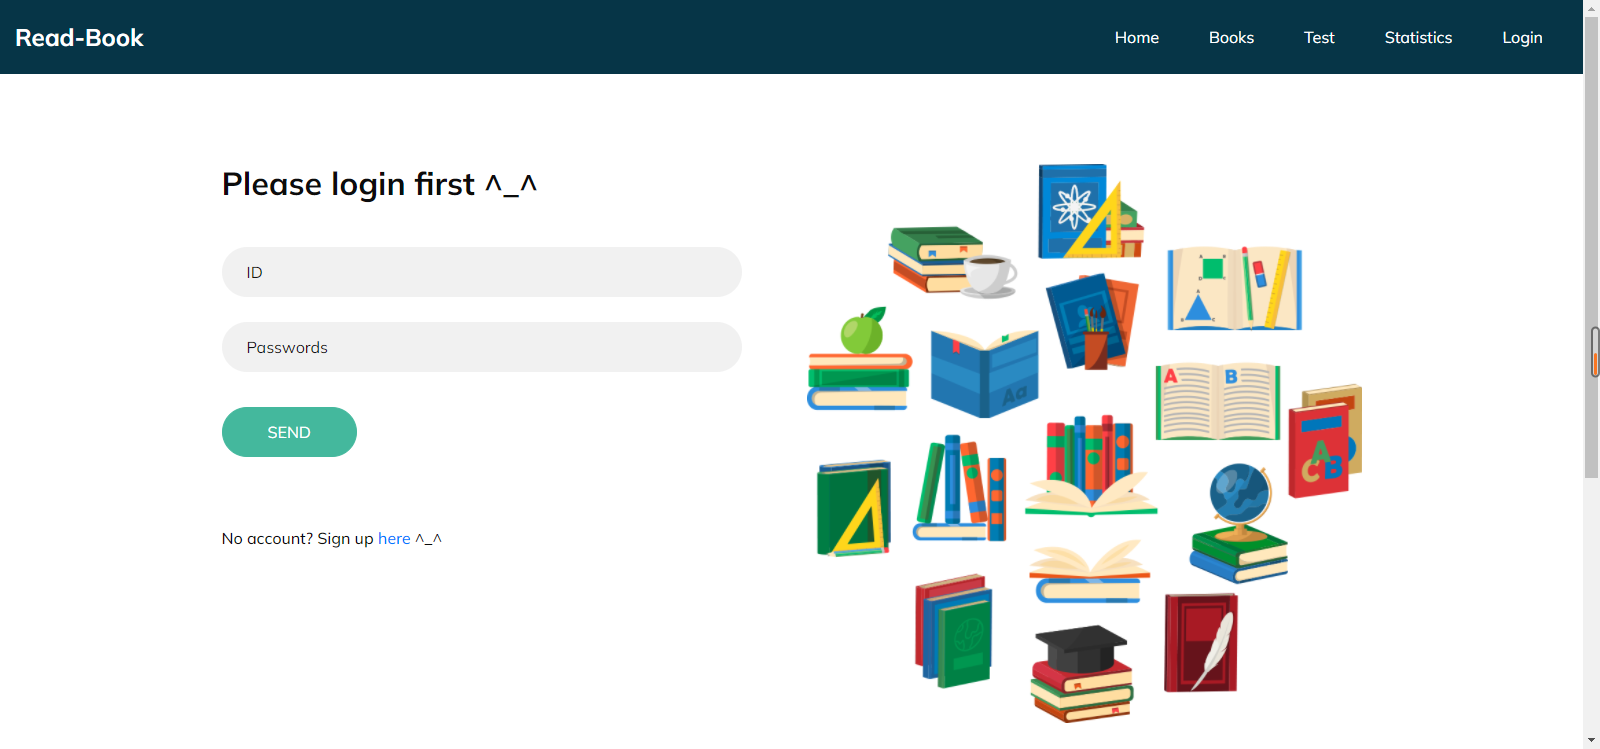
\includegraphics[width=0.9\columnwidth]{figures/login.png}
        \caption{Login}\label{fig:login}
    \end{minipage}
    \begin{minipage}[t]{0.5\linewidth}
        \centering
        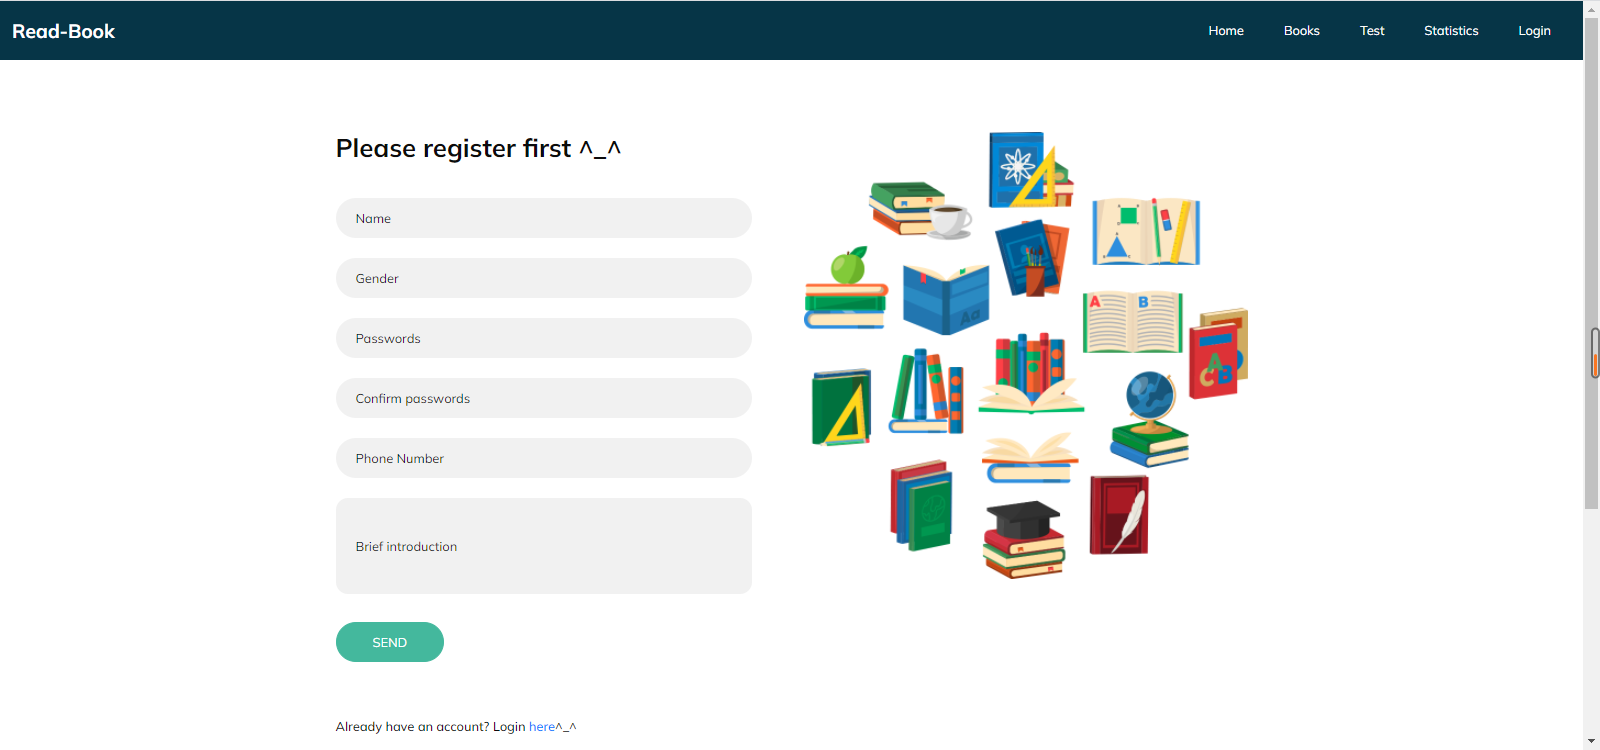
\includegraphics[width=0.9\columnwidth]{figures/reg.png}
        \caption{Register}\label{fig:reg}
    \end{minipage}
\end{figure}

\begin{figure}[H]
    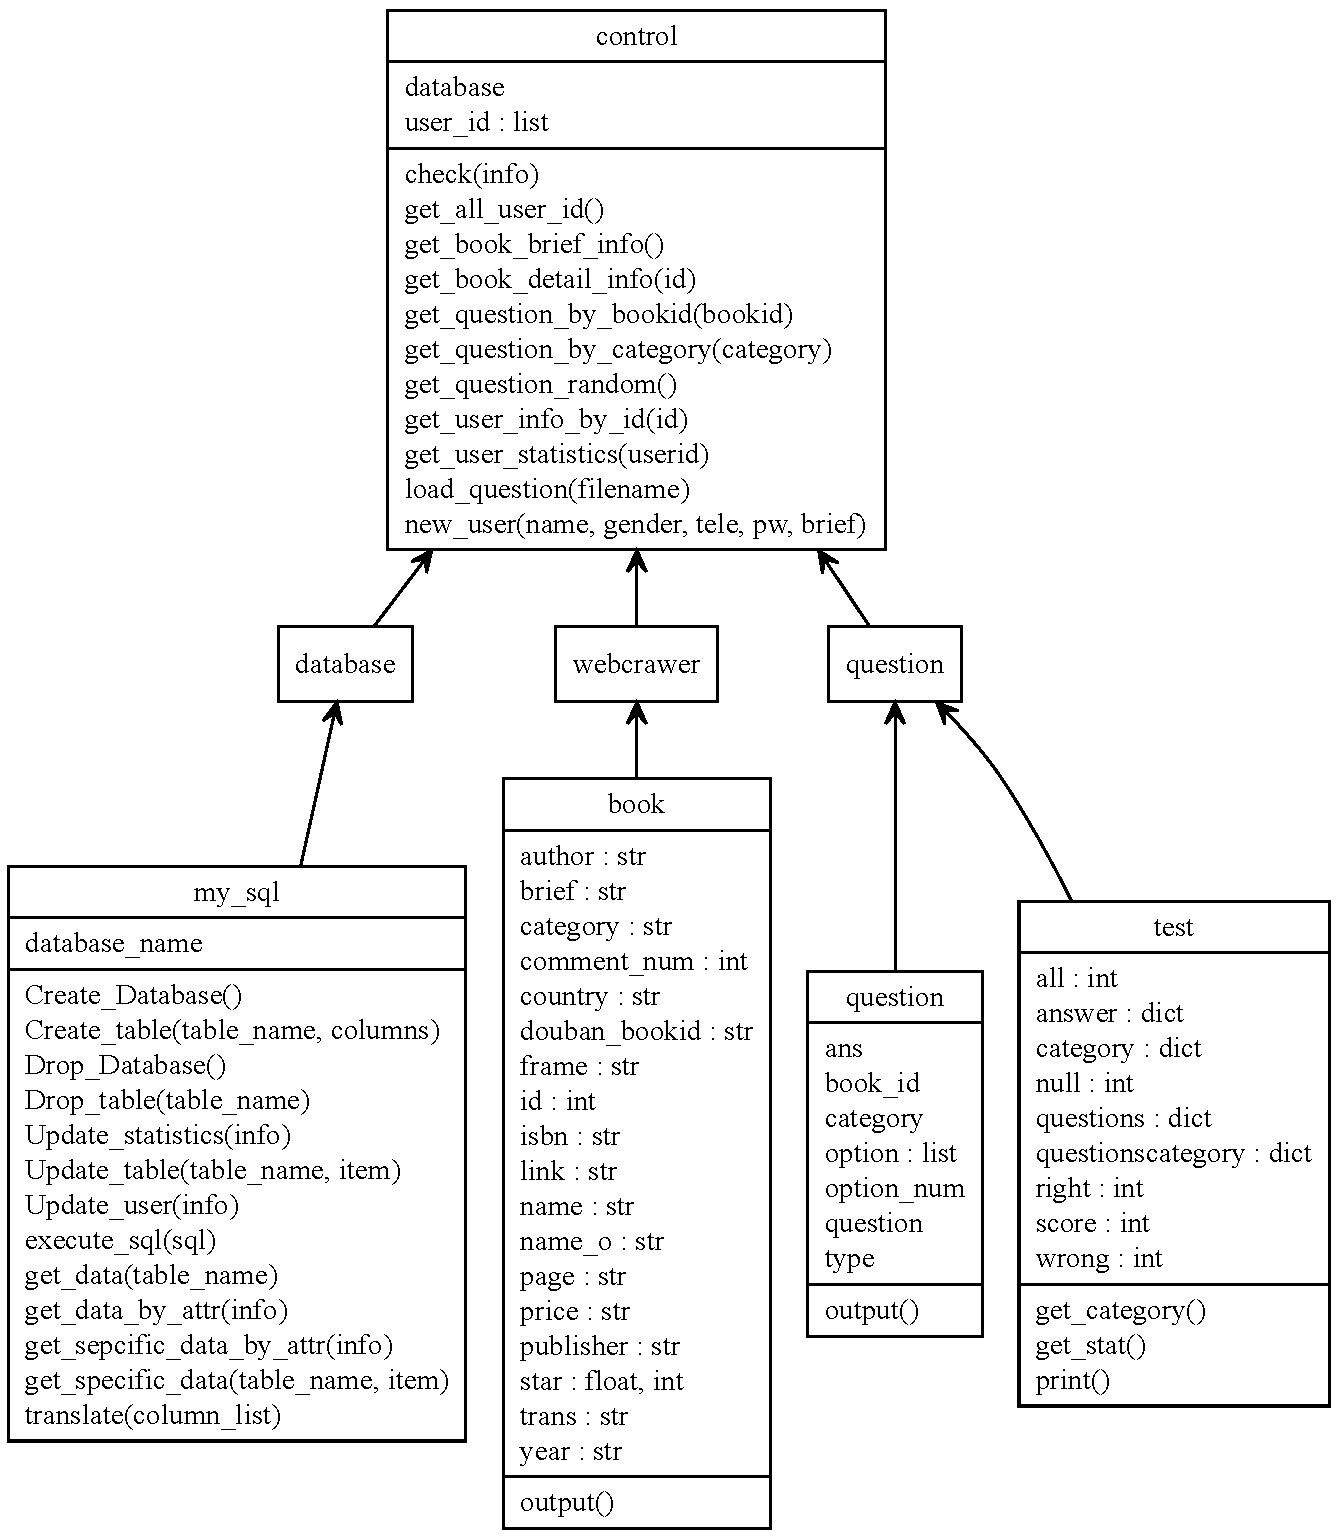
\includegraphics[width=1\columnwidth]{figures/backenduml.pdf}
    \caption{Backend UML Diagram}
    \label{fig:backenduml}
\end{figure}

\subsection{Link}

\href{http://www.castamerego.com/}{\textbf{\emph{http://www.castamerego.com/}}}

\subsection{Table}

\begin{table}[H]
    \centering
    \caption{Table Demo}
    \setlength{\tabcolsep}{7mm}{% 表格列间距
        \begin{tabular}{|c|c|c|c|c|c|c|}
            \hline
            \multicolumn{2}{|c|}{\multirow{2}{*}{日期}} & \multirow{2}{*}{版本} & \multicolumn{2}{c|}{item1} & \multicolumn{2}{c|}{item2}             \\
            \cline{4-7}
            \multicolumn{2}{|c|}{}                      &                       & 2                         & 3                          & 4 & 5    \\
            \hline
            \multirow{2}{*}{序号}                       & 0                     & 1                          & 2                          & 3 & 4 & 5 \\
            \cline{2-7}
                                                        & 0                     & 1                          & 2                          & 3 & 4 & 5 \\
            \hline
        \end{tabular}
    }

    \label{tab:tabdemo}
\end{table}

\section{Format}

\subsection{Multicolum}

\begin{multicols}{2}

    Lorem ipsum dolor sit amet, consectetur adipisicing elit, sed do eiusmod tempor incididunt ut labore et dolore magna aliqua. Ut enim ad minim veniam, quis nostrud exercitation ullamco laboris nisi ut aliquip ex ea commodo consequat. Duis aute irure dolor in reprehenderit in voluptate velit esse cillum dolore eu fugiat nulla pariatur. Excepteur sint occaecat cupidatat non proident, sunt in culpa qui officia deserunt mollit anim id est laborum.

\end{multicols}

\subsection{Box}

\subsubsection{Box}

\begin{boxedlaw}{\textwidth}
    Lorem ipsum dolor sit amet, consectetur adipisicing elit, sed do eiusmod tempor incididunt ut labore et dolore magna aliqua. Ut enim ad minim veniam, quis nostrud exercitation ullamco laboris nisi ut aliquip ex ea commodo consequat. Duis aute irure dolor in reprehenderit in voluptate velit esse cillum dolore eu fugiat nulla pariatur. Excepteur sint occaecat cupidatat non proident, sunt in culpa qui officia deserunt mollit anim id est laborum.
\end{boxedlaw}

\newpage

\subsubsection{Plain Box}
\begin{center}
    \fcolorbox{black}{white}{\parbox{1\linewidth}{
            \textbf{\emph{\Large Use Case 1: Login to the System}}

            \begin{multicols}{2}

                \textbf{Primary Actor:} Homeowner

                % \textbf{Secondary Actor:}

                \textbf{Goal in context:} To login to the system.

                \textbf{Preconditions:} System must be fully configured; Homeowner must have a valid user ID and password.

                \textbf{Trigger:} Homeowner wants to login to the system.

                \textbf{Scenario:}

                \begin{enumerate}
                    \item The homeowner logs onto the \emph{SafeHome Products} website on his PC or opens the \emph{SafeHome} application on his mobile phone.
                    \item The homeowner inputs his user ID and password.
                    \item The system displays all major functionalities of the \emph{SafeHome} system.
                \end{enumerate}

                \textbf{Exception:}

                \begin{enumerate}
                    \item If the user ID or password is incorrect, the system will display an error message and ask the user to input again.
                    \item Surveillance function not configured for this system.
                    \item An alarm condition is encountered.
                \end{enumerate}

                \textbf{Priority:} Moderate priority, to be implemented after basic functions

                \textbf{When available:} Second increment

                \textbf{Frequency of use:} Frequently

                \textbf{Channel to actor:} Via the \emph{SafeHome Products} website or the \emph{SafeHome} application

                \textbf{Open issues:}

                \begin{enumerate}
                    \item Is security sufficient? 
                    \item Maybe we can add a captcha(Completely Automated Public Turing test to tell Computers and Humans Apart) to the login page.
                    \item When client commucating with server, the ID and password should be encrypted.
                \end{enumerate}

            \end{multicols}}}
\end{center}


\vskip 0.2in

\phantomsection\addcontentsline{toc}{section}{Reference}\tolerance=500
\bibliography{references/references}

\end{document}
